% =================================================================
%  contenido.tex – Cuerpo del Reporte Técnico (PIA-ML)
%  Clasificación de Gestos (Piedra, Papel o Tijera) mediante CNN
% =================================================================

\section{Introducción}

El reconocimiento automático de gestos humanos constituye una de las líneas de investigación más activas dentro de la visión por computadora y la interacción humano--computadora (\textit{Human--Computer Interaction}, HCI). A diferencia de los periféricos convencionales como el teclado o el ratón, la comunicación gestual ofrece una interfaz natural, sin contacto físico y altamente intuitiva con aplicaciones directas en robótica colaborativa, rehabilitación médica, traducción de lengua de señas, realidad aumentada y sistemas embebidos de control industrial.

Tradicionalmente, los sistemas de visión artificial dependían de la extracción manual de descriptores visuales (\textit{hand-crafted features}) tales como bordes de Canny, histogramas de gradientes orientados (HOG) o transformaciones invariantes a escala (SIFT), acoplados a clasificadores clásicos como máquinas de soporte vectorial (SVM) o árboles de decisión. Sin embargo, dichos enfoques presentan fragilidad ante cambios en la iluminación, rotaciones de la mano, variaciones anatómicas entre individuos y ligeras oclusiones de los dedos.

El surgimiento del aprendizaje profundo (\textit{Deep Learning}), y en particular de las \textbf{Redes Neuronales Convolucionales (CNN)}, transformó radicalmente el procesamiento de imágenes al permitir que el propio modelo aprenda jerarquías automáticas de características visuales directamente desde los píxeles crudos \cite{LeCun1998, Krizhevsky2012, Goodfellow2016}. En las primeras capas, los filtros convolucionales responden a primitivas geométricas simples (bordes, gradientes de color y esquinas); en las capas intermedias y profundas, estas activaciones se combinan para representar estructuras semánticas complejas como contornos de dedos, bifurcaciones y la morfología global de la mano.

El presente proyecto final tiene como objetivo diseñar, implementar desde cero, entrenar y evaluar críticamente una Red Neuronal Convolucional capaz de clasificar imágenes de manos humanas en tres categorías de gestos correspondientes al juego clásico de \textbf{Piedra, Papel o Tijera}, utilizando el conjunto de datos público \textit{Rock, Paper, Scissors} de Kaggle \cite{Freeman2019}. Sin recurrir a modelos preentrenados ni transferencia de aprendizaje, se evalúa el desempeño de dos arquitecturas construidas íntegramente desde cero en TensorFlow/Keras \cite{Abadi2015, Chollet2021}, documentando todo el flujo experimental en una libreta ejecutable de Google Colab y analizando con rigor tanto las métricas cuantitativas como los patrones visuales de error del modelo.

\section{Antecedentes}

\subsection{Fundamentos de las Redes Neuronales Convolucionales}

Una Red Neuronal Convolucional (CNN) es una arquitectura especializada de red neuronal profunda diseñada para procesar datos con topología de cuadrícula, como imágenes digitales bidimensionales representadas por tensores tridimensionales $X \in \mathbb{R}^{H \times W \times C}$, donde $H$ es la altura, $W$ la anchura y $C$ el número de canales cromáticos ($C = 3$ para imágenes RGB) \cite{Goodfellow2016}. A diferencia de los perceptrones multicapa (MLP) tradicionales —donde cada neurona se conecta densamente con todos los píxeles de entrada, generando una explosión combinatoria de parámetros y perdiendo la estructura espacial—, las CNN explotan tres propiedades inductivas fundamentales \cite{LeCun1998}:

\begin{itemize}
    \item \textbf{Conectividad local (\textit{sparse interactions}):} cada neurona convolucional procesa únicamente una pequeña vecindad espacial o campo receptivo definido por el tamaño del núcleo (\textit{kernel}), típicamente $3 \times 3$.
    \item \textbf{Compartición de parámetros (\textit{parameter sharing}):} un mismo filtro de pesos se desliza sobre toda la imagen, reduciendo drásticamente el número de parámetros entrenables y detectando el mismo patrón independientemente de su ubicación.
    \item \textbf{Equivarianza a la traslación:} si un gesto se desplaza dentro del encuadre, su mapa de características correspondiente experimenta el mismo desplazamiento.
\end{itemize}

\subsection{Operaciones Principales de una CNN}

\subsubsection{Capa Convolucional (\texttt{Conv2D})}
Dada una entrada $X$ y un banco de $K$ filtros tridimensionales $W^{(k)} \in \mathbb{R}^{k_h \times k_w \times C}$ con sesgo $b^{(k)} \in \mathbb{R}$, el valor del mapa de características de salida $Z^{(k)}$ en la posición espacial $(i, j)$ se calcula mediante correlación cruzada discreta \cite{Goodfellow2016}:
\begin{equation}
    Z^{(k)}_{i,j} = b^{(k)} + \sum_{c=1}^{C} \sum_{m=0}^{k_h-1} \sum_{n=0}^{k_w-1} X_{i+m,\, j+n,\, c} \cdot W^{(k)}_{m,n,c}.
\end{equation}
El uso de relleno cero (\texttt{padding="same"}) preserva las dimensiones espaciales $(H, W)$ en la salida de la convolución, evitando que la información de los bordes de la imagen desaparezca prematuramente.

\subsubsection{Función de Activación No Lineal (\texttt{ReLU})}
Para dotar a la red de capacidad de aproximación no lineal, cada mapa convolucional se transforma elemento a elemento mediante la unidad lineal rectificada (\textit{Rectified Linear Unit}, ReLU) \cite{Krizhevsky2012, He2015}:
\begin{equation}
    \text{ReLU}(z) = \max(0, z).
\end{equation}
ReLU mitiga el desvanecimiento del gradiente en regiones positivas, acelera la convergencia frente a funciones sigmoidales clásicas e induce representaciones dispersas computacionalmente eficientes.

\subsubsection{Agrupación Espacial (\texttt{MaxPooling2D})}
Las capas de agrupación máxima reducen progresivamente la resolución espacial seleccionando el valor máximo dentro de ventanas locales de tamaño $2 \times 2$ con paso (\textit{stride}) $2$:
\begin{equation}
    P^{(k)}_{i,j} = \max_{0 \le m < 2,\; 0 \le n < 2} A^{(k)}_{2i+m,\, 2j+n}.
\end{equation}
Esta operación disminuye la carga computacional, amplía el campo receptivo efectivo de las capas posteriores y aporta invariancia local ante pequeñas traslaciones o deformaciones de la mano \cite{Chollet2021}.

\subsubsection{Aplanamiento, Capas Densas y Clasificación Multiclase (\texttt{Softmax})}
Tras la etapa de extracción jerárquica de características, el tensor tridimensional final se transforma en un vector unidimensional mediante \texttt{Flatten} y se alimenta a capas totalmente conectadas (\texttt{Dense}). Para un problema de clasificación multiclase con $M = 3$ clases mutuamente excluyentes, la capa de salida aplica la función \textit{Softmax} sobre el vector de \textit{logits} $\mathbf{o} = (o_1, o_2, o_3)$:
\begin{equation}
    \hat{y}_c = \frac{\exp(o_c)}{\sum_{j=1}^{M} \exp(o_j)}, \qquad c \in \{1, 2, 3\},
\end{equation}
produciendo una distribución de probabilidad válida ($\hat{y}_c \in (0,1)$ y $\sum_{c=1}^{M} \hat{y}_c = 1$). El entrenamiento minimiza la función de pérdida de \textbf{entropía cruzada categórica} (\texttt{categorical\_crossentropy}) sobre un lote de $N$ ejemplos con etiquetas codificadas en formato \textit{one-hot} $\mathbf{y}^{(i)}$:
\begin{equation}
    \mathcal{L}(\theta) = -\frac{1}{N} \sum_{i=1}^{N} \sum_{c=1}^{M} y^{(i)}_c \log\big(\hat{y}^{(i)}_c\big).
\end{equation}

\subsection{Optimización y Regularización en Redes Profundas}

La actualización iterativa de los parámetros $\theta$ se realiza mediante el optimizador \textbf{Adam} (\textit{Adaptive Moment Estimation}) \cite{Kingma2015}, el cual mantiene estimaciones móviles exponenciales del primer momento (media) y segundo momento no centrado (varianza) de los gradientes, adaptando de forma automática la tasa de aprendizaje efectiva para cada peso.

Para prevenir el sobreajuste (\textit{overfitting}) cuando el tamaño del conjunto de entrenamiento es moderado, la literatura recomienda combinar tres mecanismos complementarios:
\begin{enumerate}
    \item \textbf{Normalización por lotes (\textit{Batch Normalization}):} estandariza las activaciones intermedias por canal durante el entrenamiento, estabilizando las distribuciones internas y acelerando la optimización \cite{Ioffe2015}.
    \item \textbf{\textit{Dropout}:} desactiva estocásticamente una fracción $p$ de las neuronas densas en cada paso de entrenamiento, reduciendo la coadaptación entre características \cite{Srivastava2014}.
    \item \textbf{Aumento de datos (\textit{Data Augmentation}):} aplica transformaciones geométricas aleatorias (volteo horizontal, rotaciones moderadas y escalado) exclusivamente sobre el conjunto de entrenamiento para simular variabilidad postural sin introducir fuga de datos \cite{Chollet2021}.
\end{enumerate}

\section{Metodología}

\subsection{Descripción y Auditoría del Dataset}

Se utilizó el conjunto de datos público \textit{Rock, Paper, Scissors} disponible en Kaggle (\texttt{drgfreeman/rockpaperscissors}) \cite{Freeman2019}. Este dataset contiene un total de \textbf{2,188 imágenes RGB} de manos humanas realizando los tres gestos sobre un fondo verde uniforme (\textit{chroma key}) con una resolución nativa de $300 \times 200$ píxeles.

Como paso indispensable de calidad de datos, se ejecutó una auditoría automatizada sobre todos los archivos descargados mediante \texttt{kagglehub}, verificando la integridad binaria con \texttt{PIL.Image.verify()}, la presencia de valores nulos y la consistencia de dimensiones y canales cromáticos. Se confirmaron \textbf{0 archivos corruptos} y \textbf{0 etiquetas faltantes}. La distribución por clase es altamente equilibrada:
\begin{itemize}
    \item \textbf{Tijera (\texttt{scissors}):} 750 imágenes (34.3\%).
    \item \textbf{Piedra (\texttt{rock}):} 726 imágenes (33.2\%).
    \item \textbf{Papel (\texttt{paper}):} 712 imágenes (32.5\%).
\end{itemize}

\begin{figure}[H]
    \centering
    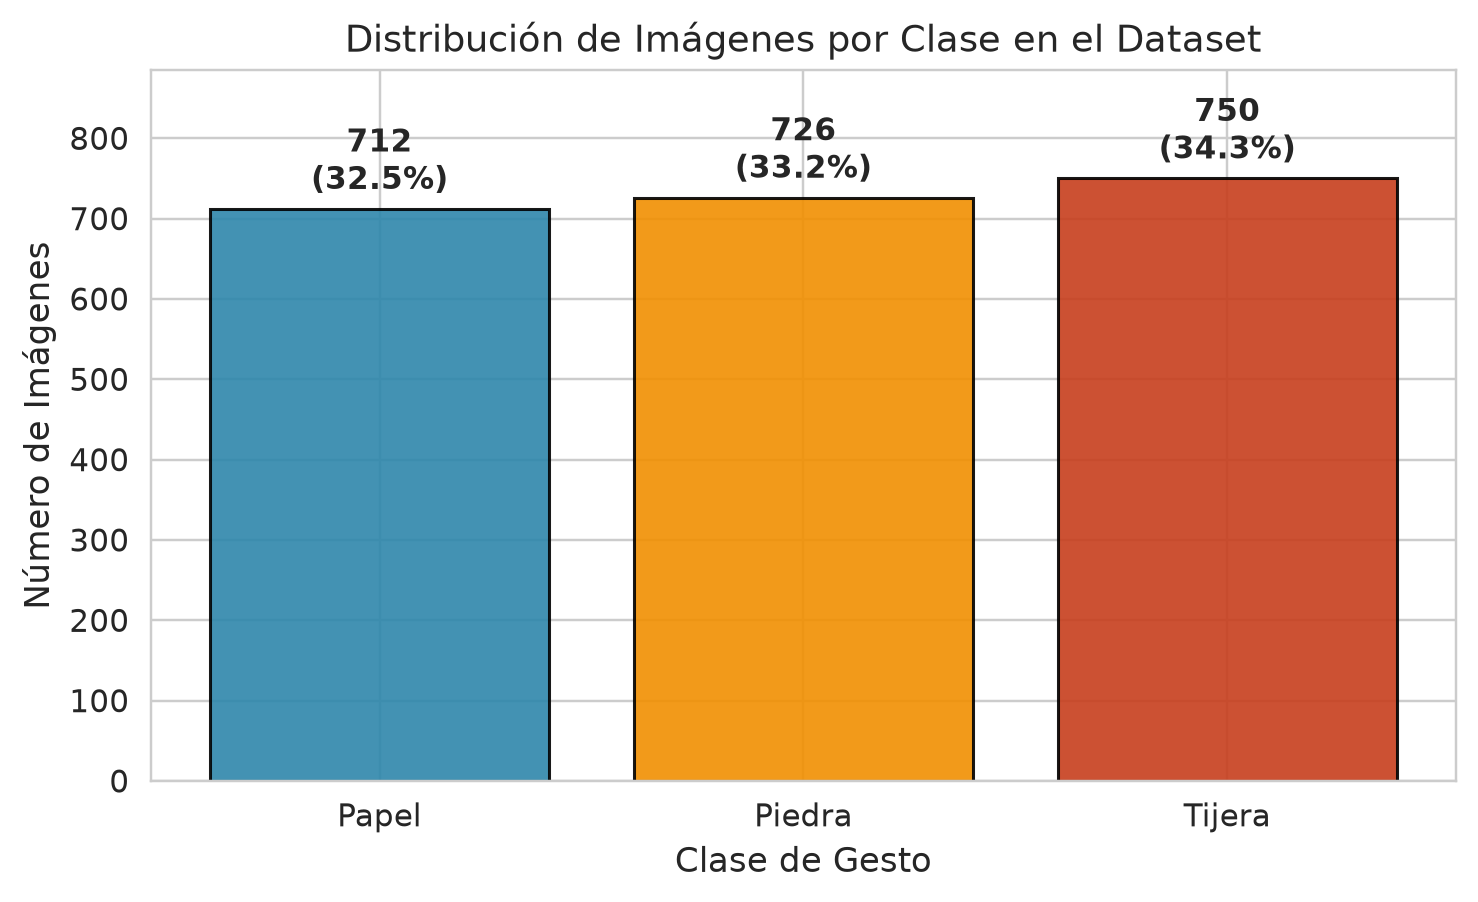
\includegraphics[width=0.72\textwidth]{Imágenes/fig_balance_clases.png}
    \caption{Distribución balanceada de las 2,188 imágenes por categoría en el dataset \textit{Rock, Paper, Scissors}.}
    \label{fig:balance_clases}
\end{figure}

\begin{figure}[H]
    \centering
    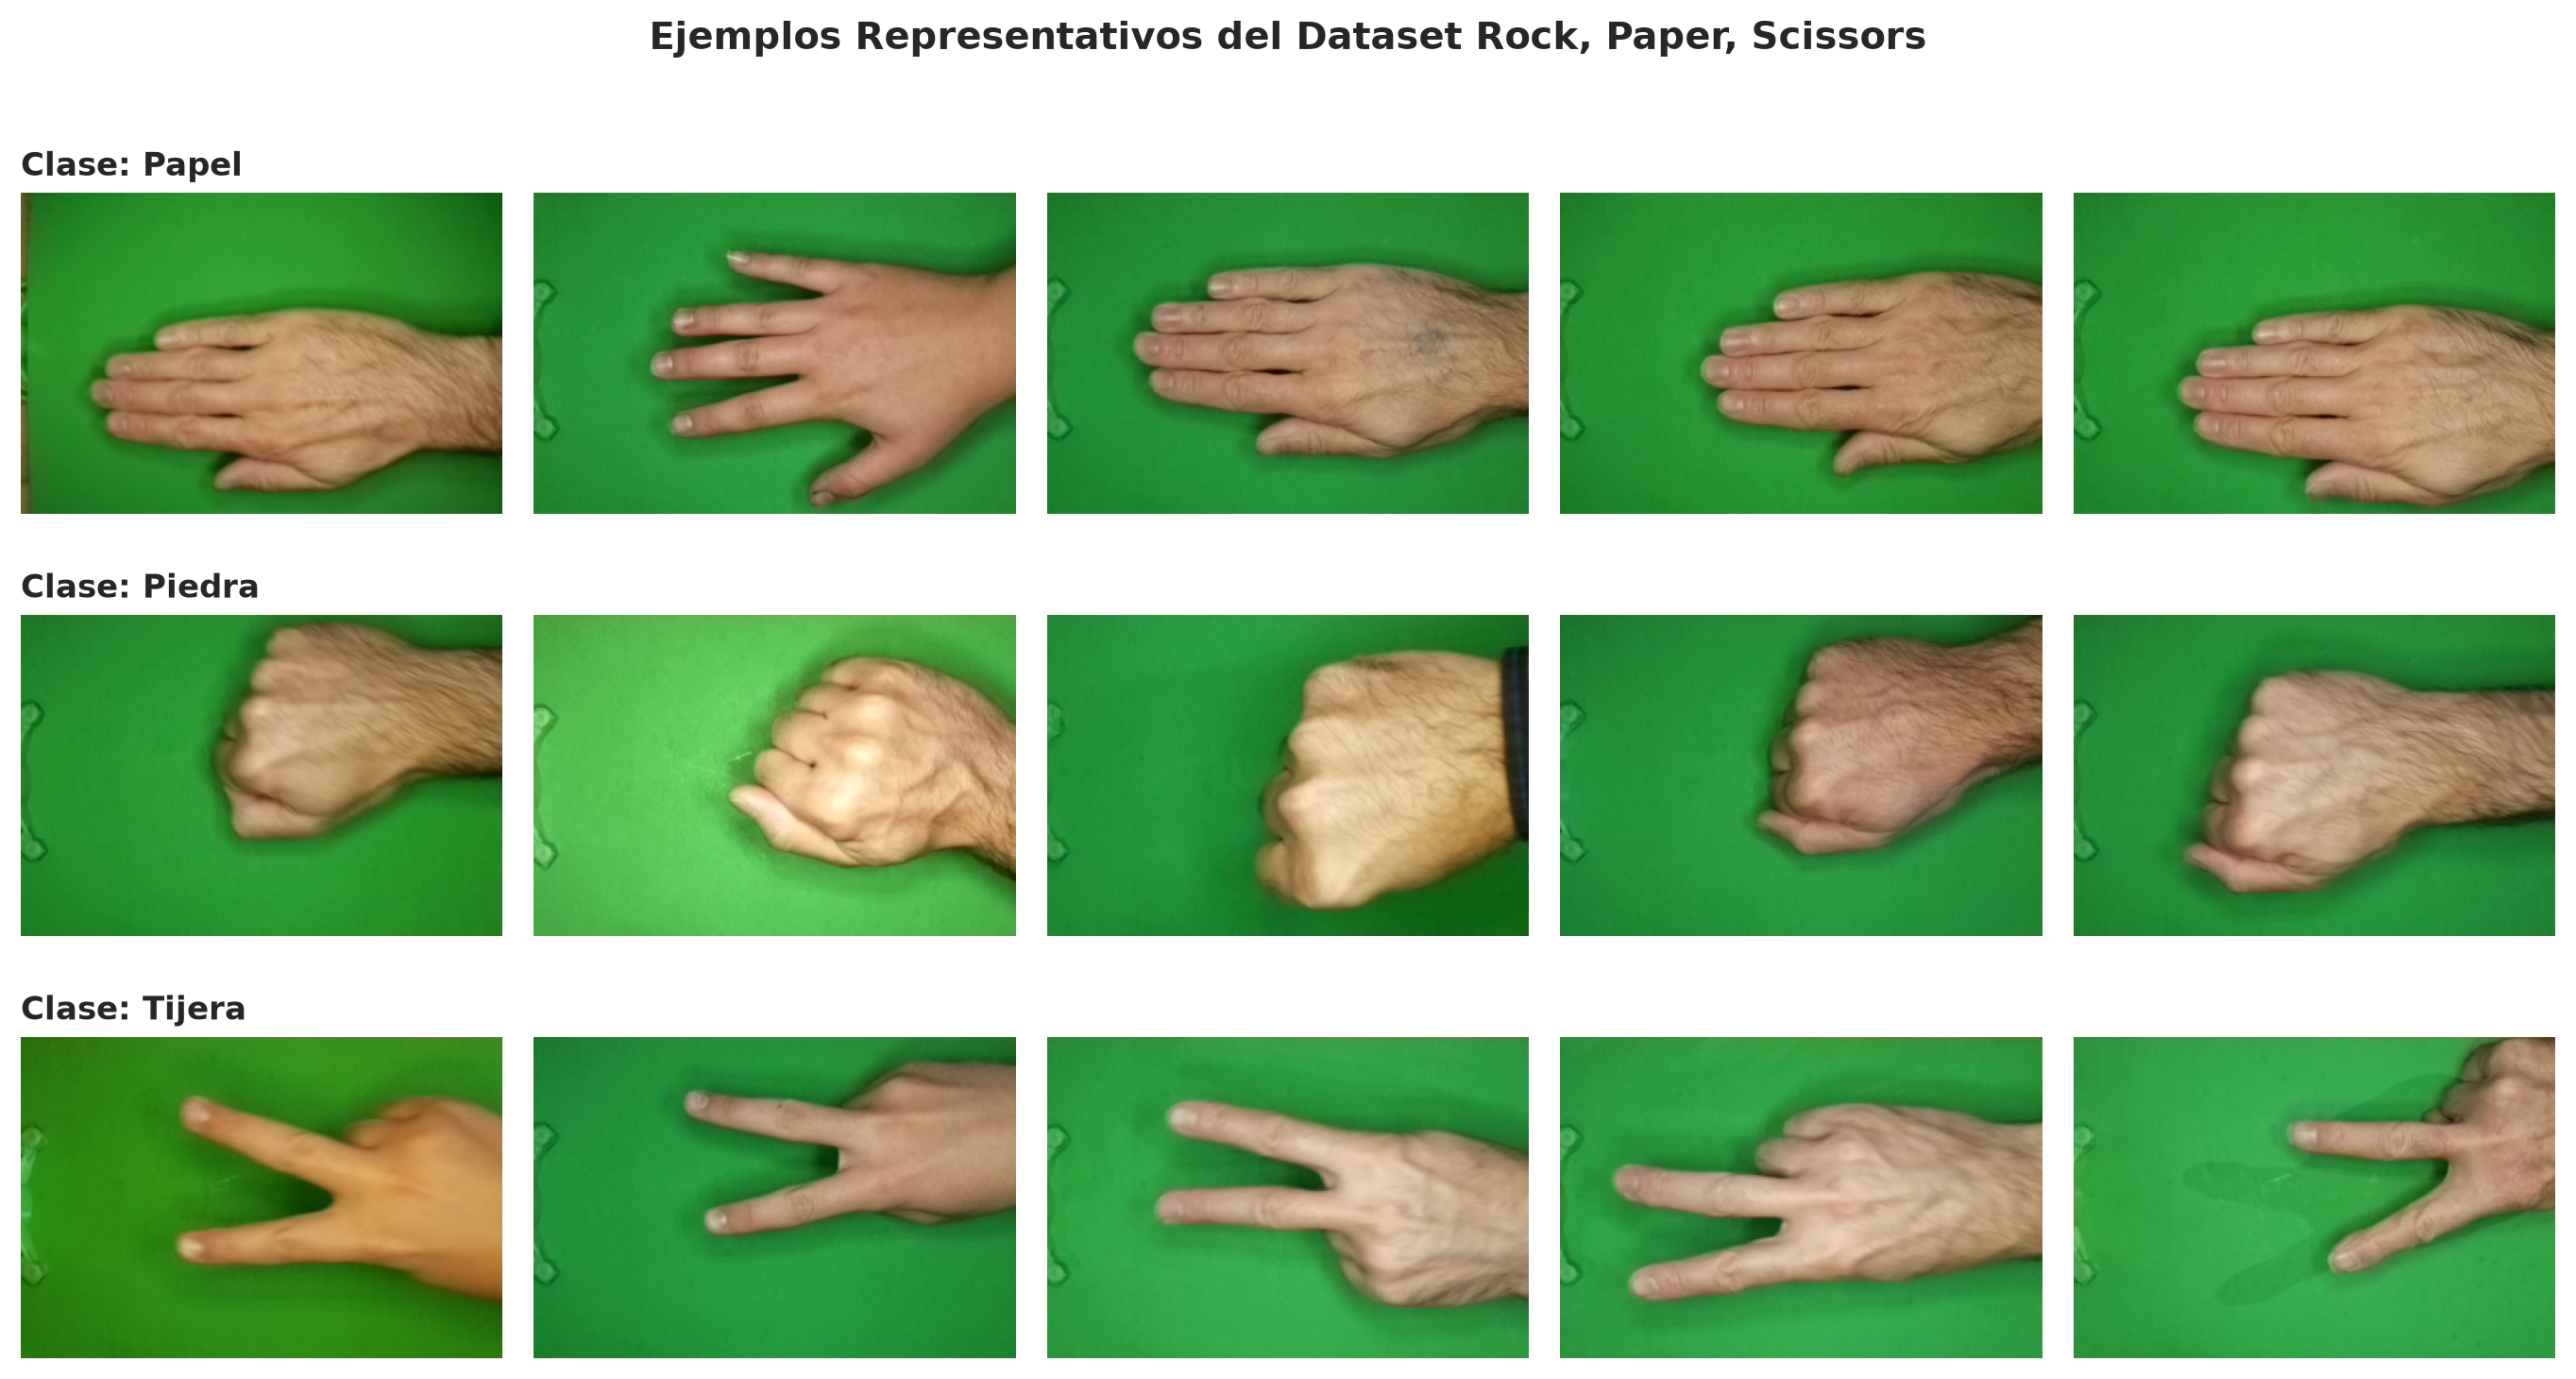
\includegraphics[width=0.98\textwidth]{Imágenes/fig_eda_muestras.png}
    \caption{Muestras representativas del conjunto de datos para las clases Papel, Piedra y Tijera.}
    \label{fig:eda_muestras}
\end{figure}

\subsection{Partición Estratificada y Preprocesamiento}

Para garantizar una evaluación libre de fuga de datos (\textit{data leakage}), la partición del conjunto se efectuó \textbf{antes} de cualquier etapa de transformación o aumento de datos, utilizando muestreo estratificado con semilla fija (\texttt{SEED = 42}) y verificación explícita de disjunción entre rutas de archivo:

\begin{table}[H]
    \centering
    \caption{Distribución estratificada de imágenes en entrenamiento, validación y prueba.}
    \label{tab:splits}
    \begin{tabular}{lcccc}
        \toprule
        \textbf{Clase} & \textbf{Train (70\%)} & \textbf{Validation (15\%)} & \textbf{Test (15\%)} & \textbf{Total} \\
        \midrule
        Papel  & 498 & 107 & 107 & 712 \\
        Piedra & 508 & 109 & 109 & 726 \\
        Tijera & 525 & 112 & 113 & 750 \\
        \midrule
        \textbf{Total} & \textbf{1,531} & \textbf{328} & \textbf{329} & \textbf{2,188} \\
        \bottomrule
    \end{tabular}
\end{table}

Cada imagen fue sometida al siguiente preprocesamiento estándar:
\begin{enumerate}
    \item \textbf{Redimensionamiento uniforme:} interpolación bilineal hacia una resolución cuadrada de $150 \times 150 \times 3$ píxeles (\texttt{RGB}), preservando los contornos de los dedos mientras se reduce el costo de memoria por lote.
    \item \textbf{Normalización de píxeles:} conversión a precisión flotante \texttt{float32} y división entre $255.0$ para mapear el rango original $[0, 255]$ al intervalo $[0, 1]$:
    \begin{equation}
        X_{\text{norm}} = \frac{X_{\text{raw}}}{255.0} \in [0, 1]^{150 \times 150 \times 3}.
    \end{equation}
    \item \textbf{Codificación de etiquetas:} representación \textit{one-hot} tridimensional compatible con \texttt{categorical\_crossentropy}.
\end{enumerate}

\subsubsection{Justificación Técnica de la Normalización de Píxeles}
En respuesta a la pregunta planteada en la Sección 1, normalizar los valores de intensidad al rango $[0, 1]$ antes de alimentar las capas convolucionales es esencial por cuatro razones numéricas y de optimización:
\begin{enumerate}
    \item \textbf{Estabilidad de gradientes:} entradas en $[0, 255]$ producen pre-activaciones y gradientes de gran magnitud durante la retropropagación, favoreciendo explosión de gradientes e inestabilidad en los pasos iniciales.
    \item \textbf{Mejor condicionamiento de la función de pérdida:} acotar las entradas genera contornos de pérdida más isotrópicos, permitiendo que Adam converja más rápido y con menores oscilaciones empleando tasas de aprendizaje estándar ($10^{-3}$).
    \item \textbf{Coherencia con la inicialización de pesos:} esquemas como Glorot/Xavier y He \cite{He2015} asumen varianza unitaria o acotada en las activaciones de entrada para preservar la escala de las señales a través de la profundidad de la red.
    \item \textbf{Prevención de saturación y homogeneidad entre canales:} mantiene los canales R, G y B en una misma escala acotada, reduciendo el riesgo de neuronas inactivas (\textit{dying ReLU}) y asegurando un efecto uniforme de la regularización.
\end{enumerate}

\subsection{Diseño de Arquitecturas CNN desde Cero}

Cumpliendo estrictamente el requisito de \textbf{no utilizar modelos preentrenados}, se diseñaron y compararon dos arquitecturas convolucionales construidas desde cero en TensorFlow/Keras:

\begin{itemize}
    \item \textbf{Arquitectura 1 — \texttt{CNN\_v1\_Base} (5,402,179 parámetros):} red secuencial clásica de tres bloques \texttt{Conv2D} (32, 64 y 128 filtros de $3 \times 3$, activación \texttt{ReLU}, \texttt{padding="same"}) seguidos de \texttt{MaxPooling2D(2×2)}, aplanamiento (\texttt{Flatten}), capa densa oculta de 128 neuronas (\texttt{ReLU}) y capa de salida \texttt{Dense(3, softmax)}.
    \item \textbf{Arquitectura 2 — \texttt{CNN\_v2\_Regularizada} (1,569,507 parámetros):} extiende la arquitectura base incorporando aumento de datos exclusivo en entrenamiento (\texttt{RandomFlip}, \texttt{RandomRotation(0.10)}, \texttt{RandomZoom(0.10)} con \texttt{fill\_mode="nearest"}), cuatro bloques \texttt{Conv2D} $\to$ \texttt{BatchNormalization(momentum=0.85)} $\to$ \texttt{ReLU} $\to$ \texttt{MaxPooling2D} (32, 64, 128 y 128 filtros) y \texttt{Dropout(0.35)} antes de la salida \texttt{Softmax}. El cuarto bloque reduce el mapa espacial de $18 \times 18$ a $9 \times 9$, disminuyendo en $3.44\times$ el total de parámetros entrenables.
\end{itemize}

\begin{figure}[H]
    \centering
    \begin{tikzpicture}[
        node distance=0.45cm,
        block/.style={rectangle, draw=blue!60!black, fill=blue!8, rounded corners=2pt, minimum width=1.65cm, minimum height=1.05cm, align=center, font=\scriptsize},
        dense/.style={rectangle, draw=orange!70!black, fill=orange!12, rounded corners=2pt, minimum width=1.55cm, minimum height=1.05cm, align=center, font=\scriptsize},
        outblk/.style={rectangle, draw=green!50!black, fill=green!12, rounded corners=2pt, minimum width=1.6cm, minimum height=1.05cm, align=center, font=\scriptsize},
        arrow/.style={-{Stealth[length=2.2mm]}, thick, draw=black!70}
    ]
        \node[block, fill=gray!12, draw=gray!60!black] (in) {\textbf{Entrada}\\$150\times150\times3$\\$[0,1]$};
        \node[block, right=of in] (b1) {\textbf{Bloque 1}\\Conv2D(32)\\MaxPool $2\times2$\\$75\times75\times32$};
        \node[block, right=of b1] (b2) {\textbf{Bloque 2}\\Conv2D(64)\\MaxPool $2\times2$\\$37\times37\times64$};
        \node[block, right=of b2] (b3) {\textbf{Bloque 3}\\Conv2D(128)\\MaxPool $2\times2$\\$18\times18\times128$};
        \node[dense, right=of b3] (fc) {\textbf{Clasificador}\\Flatten\\Dense(128)\\ReLU};
        \node[outblk, right=of fc] (out) {\textbf{Salida}\\Dense(3)\\Softmax\\(P, R, T)};

        \draw[arrow] (in) -- (b1);
        \draw[arrow] (b1) -- (b2);
        \draw[arrow] (b2) -- (b3);
        \draw[arrow] (b3) -- (fc);
        \draw[arrow] (fc) -- (out);
    \end{tikzpicture}
    \caption{Diagrama esquemático de la arquitectura convolucional secuencial base (\texttt{CNN\_v1\_Base}) diseñada desde cero.}
    \label{fig:arquitectura_cnn}
\end{figure}

\begin{table}[H]
    \centering
    \caption{Resumen comparativo de hiperparámetros de compilación y entrenamiento.}
    \label{tab:hiperparametros}
    \begin{tabular}{ll}
        \toprule
        \textbf{Hiperparámetro / Configuración} & \textbf{Valor Aplicado} \\
        \midrule
        Resolución de entrada & $150 \times 150 \times 3$ (RGB, normalizado en $[0, 1]$) \\
        Optimizador & Adam (\texttt{learning\_rate} inicial $= 1\times 10^{-3}$) \\
        Función de pérdida & \texttt{categorical\_crossentropy} \\
        Métrica principal de monitoreo & \texttt{accuracy} (complementada con Precision, Recall, F1) \\
        Tamaño de lote (\texttt{batch\_size}) & 32 imágenes \\
        Épocas máximas & 20 épocas \\
        Callbacks de regularización & \texttt{EarlyStopping(patience=6, start\_from\_epoch=5)}, \texttt{ReduceLROnPlateau(factor=0.5, patience=3)} \\
        Semilla de reproducibilidad & \texttt{SEED = 42} \\
        \bottomrule
    \end{tabular}
\end{table}

\subsection{Repositorio y Libreta Ejecutable en Google Colab}

La solución completa, incluyendo la libreta ejecutable para Google Colab, el entorno reproducible en Docker y la definición de integración continua (CI/CD), se aloja en el repositorio oficial de GitHub del curso:
\begin{itemize}
    \item \textbf{Repositorio GitHub:} \url{https://github.com/Xraight/FIME-Machine-Learning-}
    \item \textbf{Ruta de la libreta en el repositorio:} \texttt{notebooks/PIA\_CNN\_Piedra\_Papel\_Tijera.ipynb} (y en \texttt{PIA-Clasificacion-de-Gestos-CNN/PIA\_CNN\_Piedra\_Papel\_Tijera.ipynb})
    \item \textbf{Enlace directo a Google Colab:} \url{https://colab.research.google.com/github/Xraight/FIME-Machine-Learning-/blob/main/notebooks/PIA_CNN_Piedra_Papel_Tijera.ipynb}
\end{itemize}

\section{Resultados}

\subsection{Evolución del Entrenamiento y Comparativa de Arquitecturas}

Ambas arquitecturas fueron entrenadas bajo condiciones idénticas sobre el subconjunto de entrenamiento ($N_{\text{train}} = 1,531$) y monitoreadas sobre el subconjunto de validación ($N_{\text{val}} = 328$). La Tabla~\ref{tab:comparativa_modelos} sintetiza el desempeño cuantitativo de ambos modelos construidos desde cero.

\begin{table}[H]
    \centering
    \caption{Comparativa cuantitativa entre las arquitecturas CNN diseñadas desde cero.}
    \label{tab:comparativa_modelos}
    \begin{tabular}{lcccccc}
        \toprule
        \textbf{Modelo} & \textbf{Parámetros} & \textbf{Épocas} & \textbf{Val Loss} & \textbf{Val Acc} & \textbf{Test Loss} & \textbf{Test Acc} \\
        \midrule
        \texttt{CNN\_v1\_Base}         & 5,402,179 & 14 & 0.0646 & 98.17\% & 0.0469 & \textbf{99.39\%} \\
        \texttt{CNN\_v2\_Regularizada} & \textbf{1,569,507} & 20 & \textbf{0.0065} & \textbf{99.70\%} & \textbf{0.0180} & 98.78\% \\
        \bottomrule
    \end{tabular}
\end{table}

El criterio objetivo de selección de modelo basado exclusivamente en el conjunto de validación eligió a \textbf{\texttt{CNN\_v2\_Regularizada}}, al alcanzar una precisión de validación del \textbf{99.70\%} ($327/328$ aciertos) y una pérdida de validación de tan solo $0.0065$, reduciendo además en \textbf{$3.44\times$} el número de parámetros entrenables frente a \texttt{CNN\_v1\_Base}. Al evaluarse sobre el conjunto de prueba independiente ($N_{\text{test}} = 329$), \texttt{CNN\_v2\_Regularizada} obtuvo una precisión final de \textbf{98.78\%} ($325/329$ aciertos) y la menor pérdida de entropía cruzada en prueba (\textbf{$\mathcal{L}_{\text{test}} = 0.0180$}, $2.6\times$ inferior a la de \texttt{CNN\_v1\_Base}), mientras que \texttt{CNN\_v1\_Base} alcanzó \textbf{99.39\%} ($327/329$ aciertos) con $\mathcal{L}_{\text{test}} = 0.0469$.

\begin{figure}[H]
    \centering
    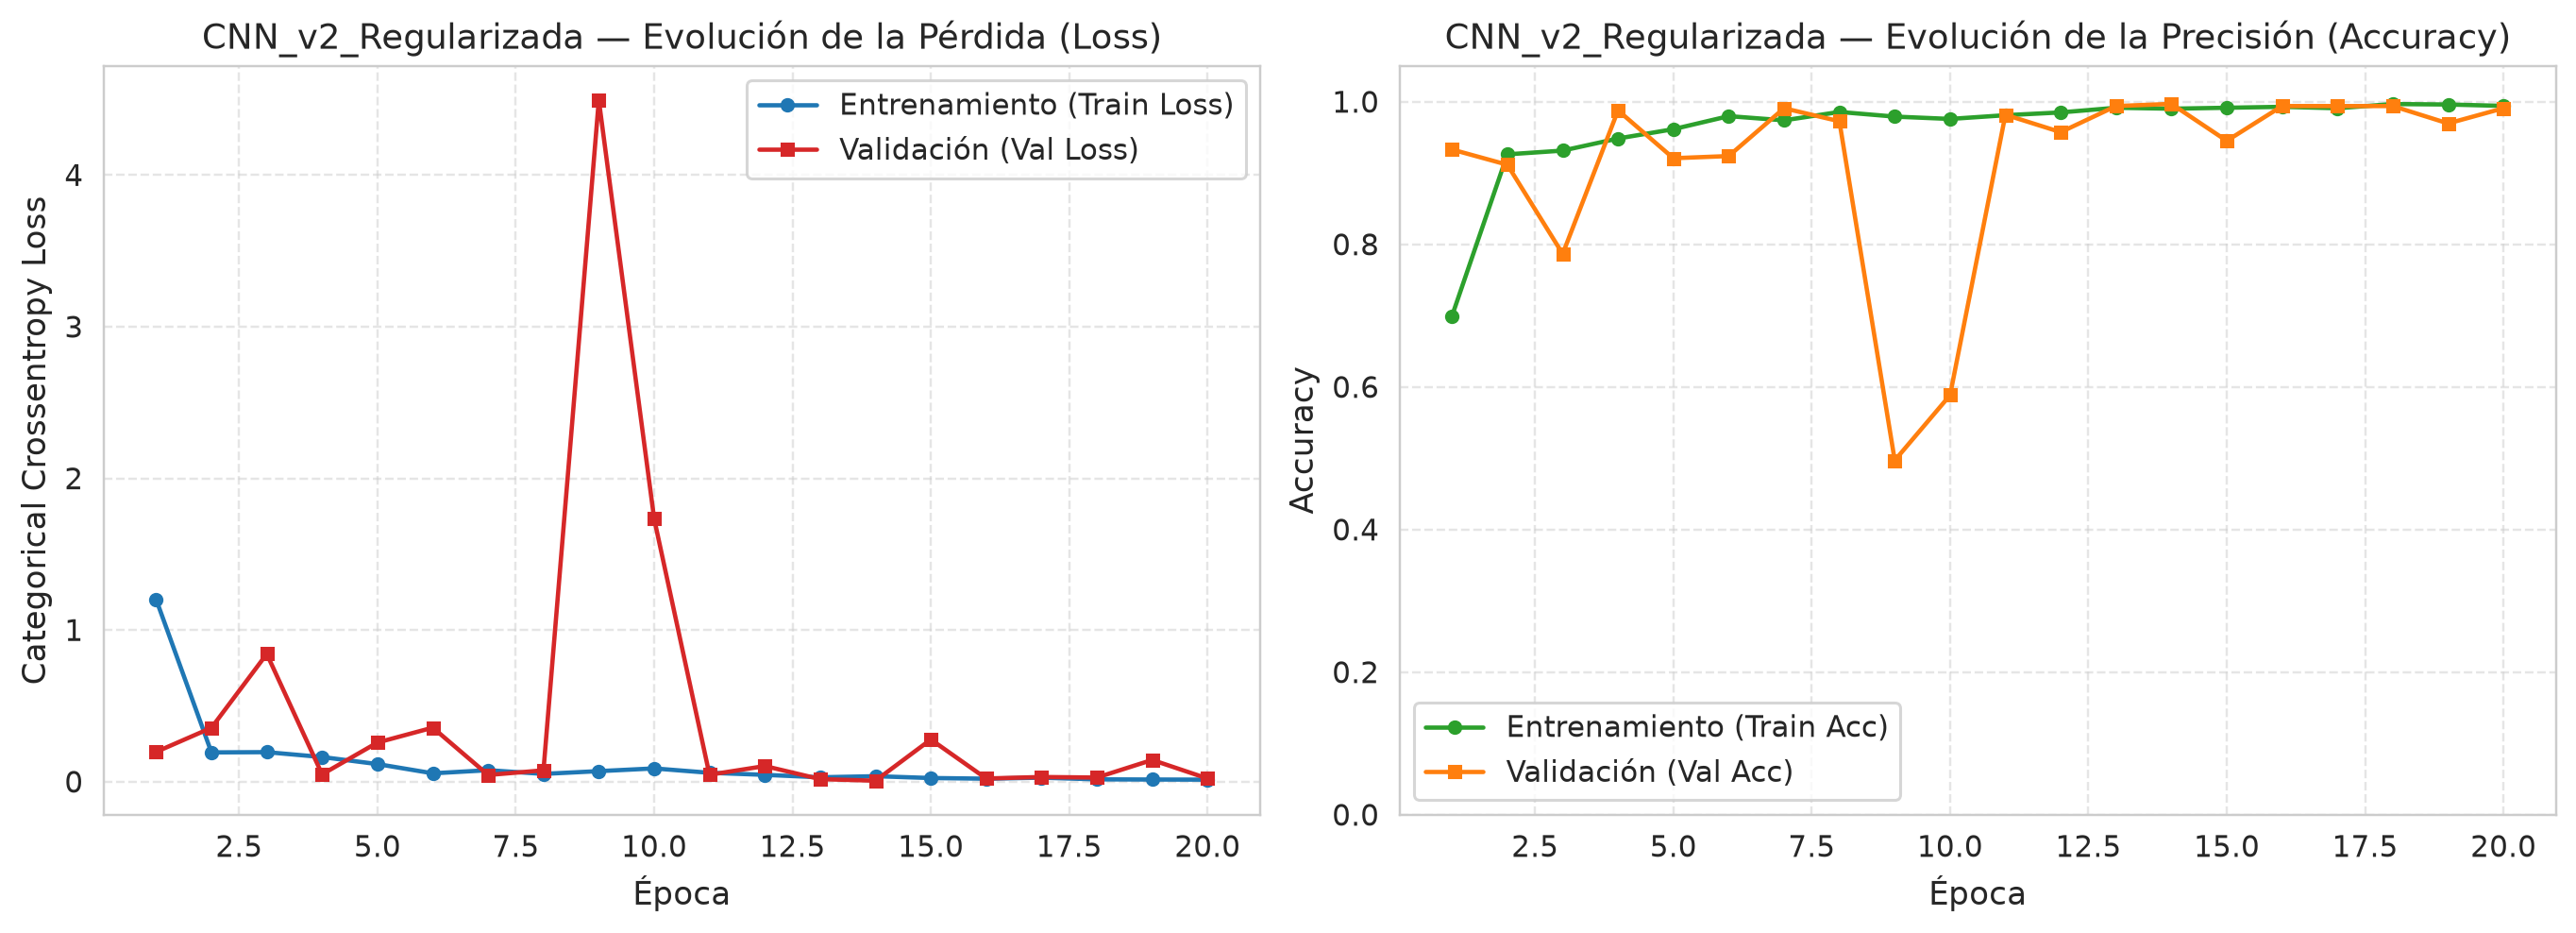
\includegraphics[width=0.98\textwidth]{Imágenes/fig_curvas_aprendizaje.png}
    \caption{Curvas de evolución de pérdida (\textit{Loss}) y precisión (\textit{Accuracy}) en entrenamiento y validación para el modelo seleccionado (\texttt{CNN\_v2\_Regularizada}).}
    \label{fig:curvas_aprendizaje}
\end{figure}

\begin{figure}[H]
    \centering
    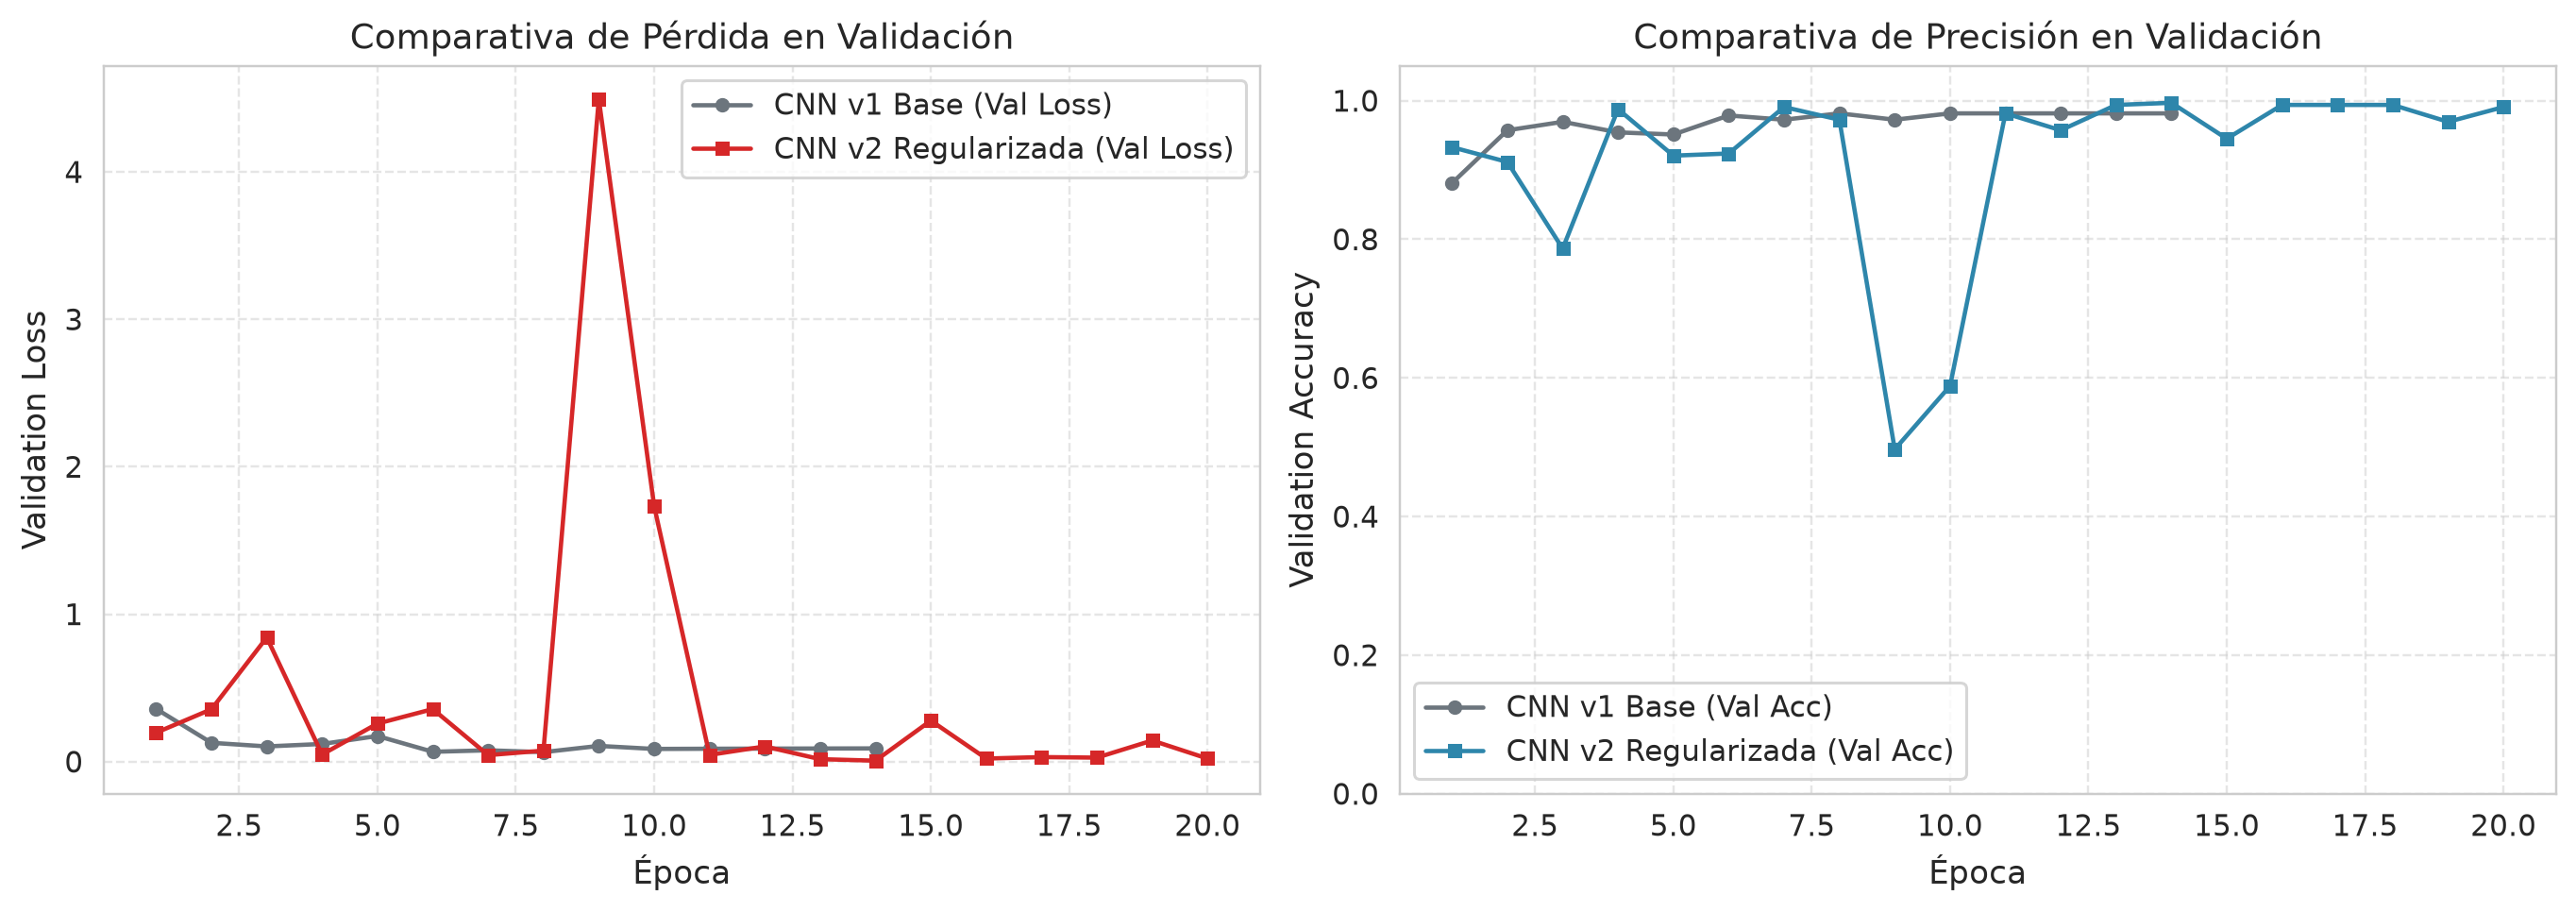
\includegraphics[width=0.98\textwidth]{Imágenes/fig_comparativa_modelos.png}
    \caption{Comparación directa de pérdida y precisión en el conjunto de validación entre \texttt{CNN\_v1\_Base} y \texttt{CNN\_v2\_Regularizada}.}
    \label{fig:comparativa_modelos}
\end{figure}

Como se aprecia en las Figuras~\ref{fig:curvas_aprendizaje} y~\ref{fig:comparativa_modelos}, \texttt{CNN\_v2\_Regularizada} experimenta una oscilación transitoria alrededor de la época 9 asociada a la interacción entre las rotaciones estocásticas del aumento de datos y las estadísticas móviles de \texttt{BatchNormalization}; sin embargo, la reducción automática de la tasa de aprendizaje (\texttt{ReduceLROnPlateau}) estabiliza rápidamente la trayectoria a partir de la época 11, convergiendo hacia una pérdida de validación virtualmente nula ($\mathcal{L}_{\text{val}} = 0.0065$) sin síntomas de sobreajuste.

\subsection{Matriz de Confusión y Métricas de Evaluación por Clase}

La Figura~\ref{fig:matriz_confusion} presenta la matriz de confusión en conteos absolutos y porcentajes normalizados por fila sobre las $329$ imágenes del conjunto de prueba para \texttt{CNN\_v2\_Regularizada}, y la Tabla~\ref{tab:reporte_clasificacion} detalla las métricas de \textit{Precision}, \textit{Recall} y \textit{F1-score} por categoría.

\begin{figure}[H]
    \centering
    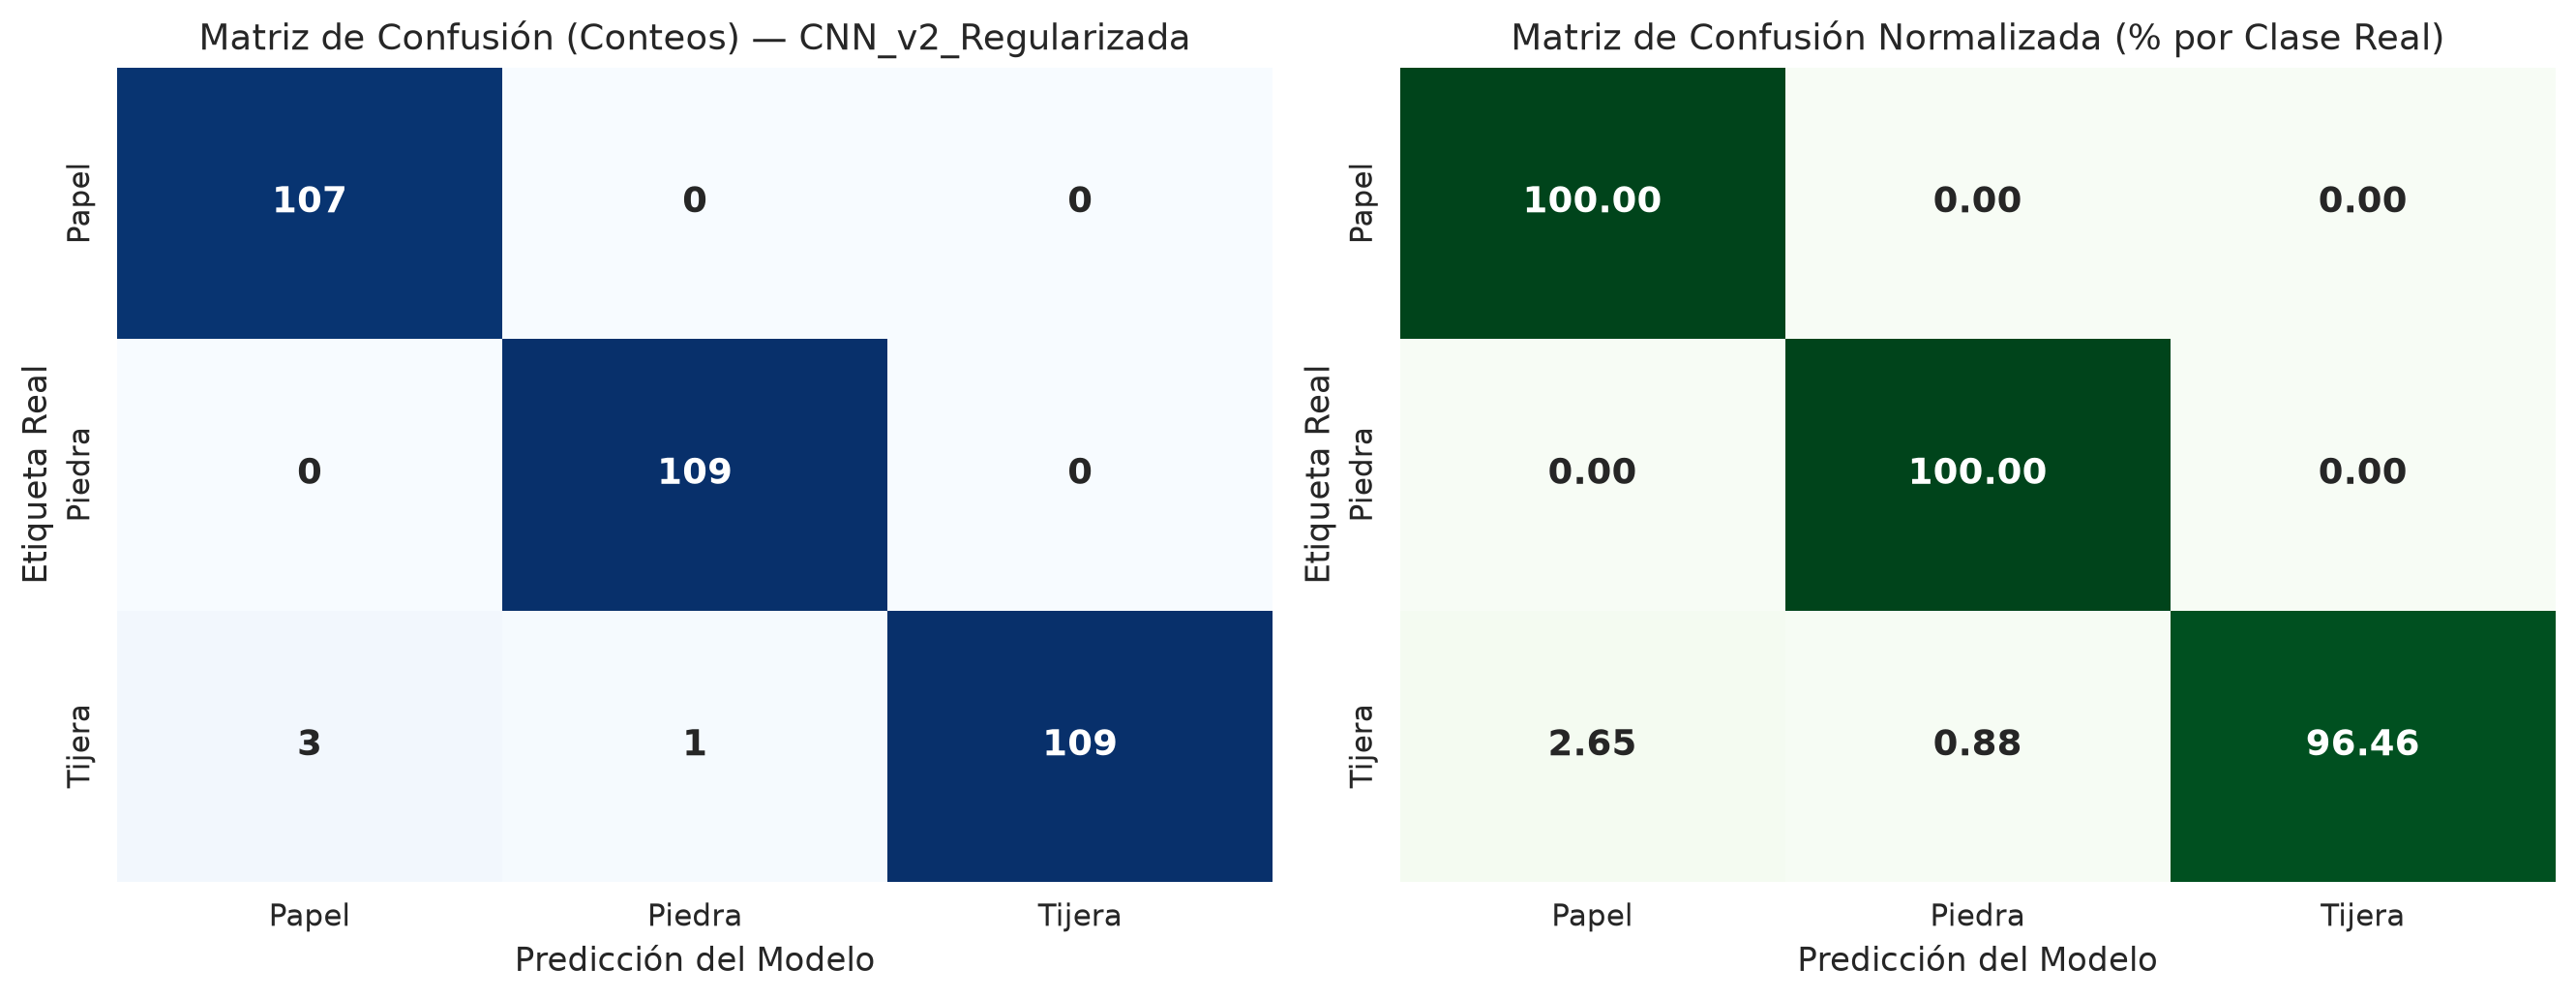
\includegraphics[width=0.98\textwidth]{Imágenes/fig_matriz_confusion.png}
    \caption{Matriz de confusión en el conjunto de prueba ($N_{\text{test}} = 329$): conteos absolutos (izquierda) y porcentajes normalizados por clase real (derecha).}
    \label{fig:matriz_confusion}
\end{figure}

\begin{table}[H]
    \centering
    \caption{Reporte detallado de clasificación sobre el conjunto de prueba (\texttt{CNN\_v2\_Regularizada}).}
    \label{tab:reporte_clasificacion}
    \begin{tabular}{lcccc}
        \toprule
        \textbf{Clase / Promedio} & \textbf{Precision} & \textbf{Recall} & \textbf{F1-Score} & \textbf{Soporte ($N$)} \\
        \midrule
        Papel  & 0.9727 & 1.0000 & 0.9862 & 107 \\
        Piedra & 0.9909 & 1.0000 & 0.9954 & 109 \\
        Tijera & 1.0000 & 0.9646 & 0.9820 & 113 \\
        \midrule
        \textbf{Exactitud global (Accuracy)} & \multicolumn{3}{c}{\textbf{0.9878 (98.78\%)}} & \textbf{329} \\
        Promedio Macro (\textit{Macro Avg}) & 0.9879 & 0.9882 & 0.9879 & 329 \\
        Promedio Ponderado (\textit{Weighted Avg}) & 0.9881 & 0.9878 & 0.9878 & 329 \\
        \bottomrule
    \end{tabular}
\end{table}

Los resultados por clase demuestran un desempeño sobresaliente y equilibrado:
\begin{itemize}
    \item \textbf{Piedra:} alcanza un \textit{Recall} del $100.0\%$ ($109/109$), \textit{Precision} de $99.09\%$ y el mayor \textit{F1-score} del sistema ($99.54\%$).
    \item \textbf{Papel:} obtiene un \textit{Recall} del $100.0\%$ ($107/107$ correctamente identificados) y un \textit{F1-score} de $98.62\%$.
    \item \textbf{Tijera:} logra una \textit{Precision} perfecta del $100.0\%$ (cero falsos positivos hacia Tijera) y un \textit{Recall} de $96.46\%$ ($109/113$ aciertos).
\end{itemize}

\subsection{Inspección Visual de Aciertos y Errores}

La Figura~\ref{fig:aciertos} muestra nueve ejemplos representativos del conjunto de prueba clasificados correctamente por la red con niveles de confianza cercanos al $100\%$. Por su parte, la Figura~\ref{fig:errores} expone la totalidad de los cuatro errores cometidos por \texttt{CNN\_v2\_Regularizada} en las $329$ imágenes de prueba, indicando tanto la probabilidad asignada a la etiqueta real como a la clase predicha.

\begin{figure}[H]
    \centering
    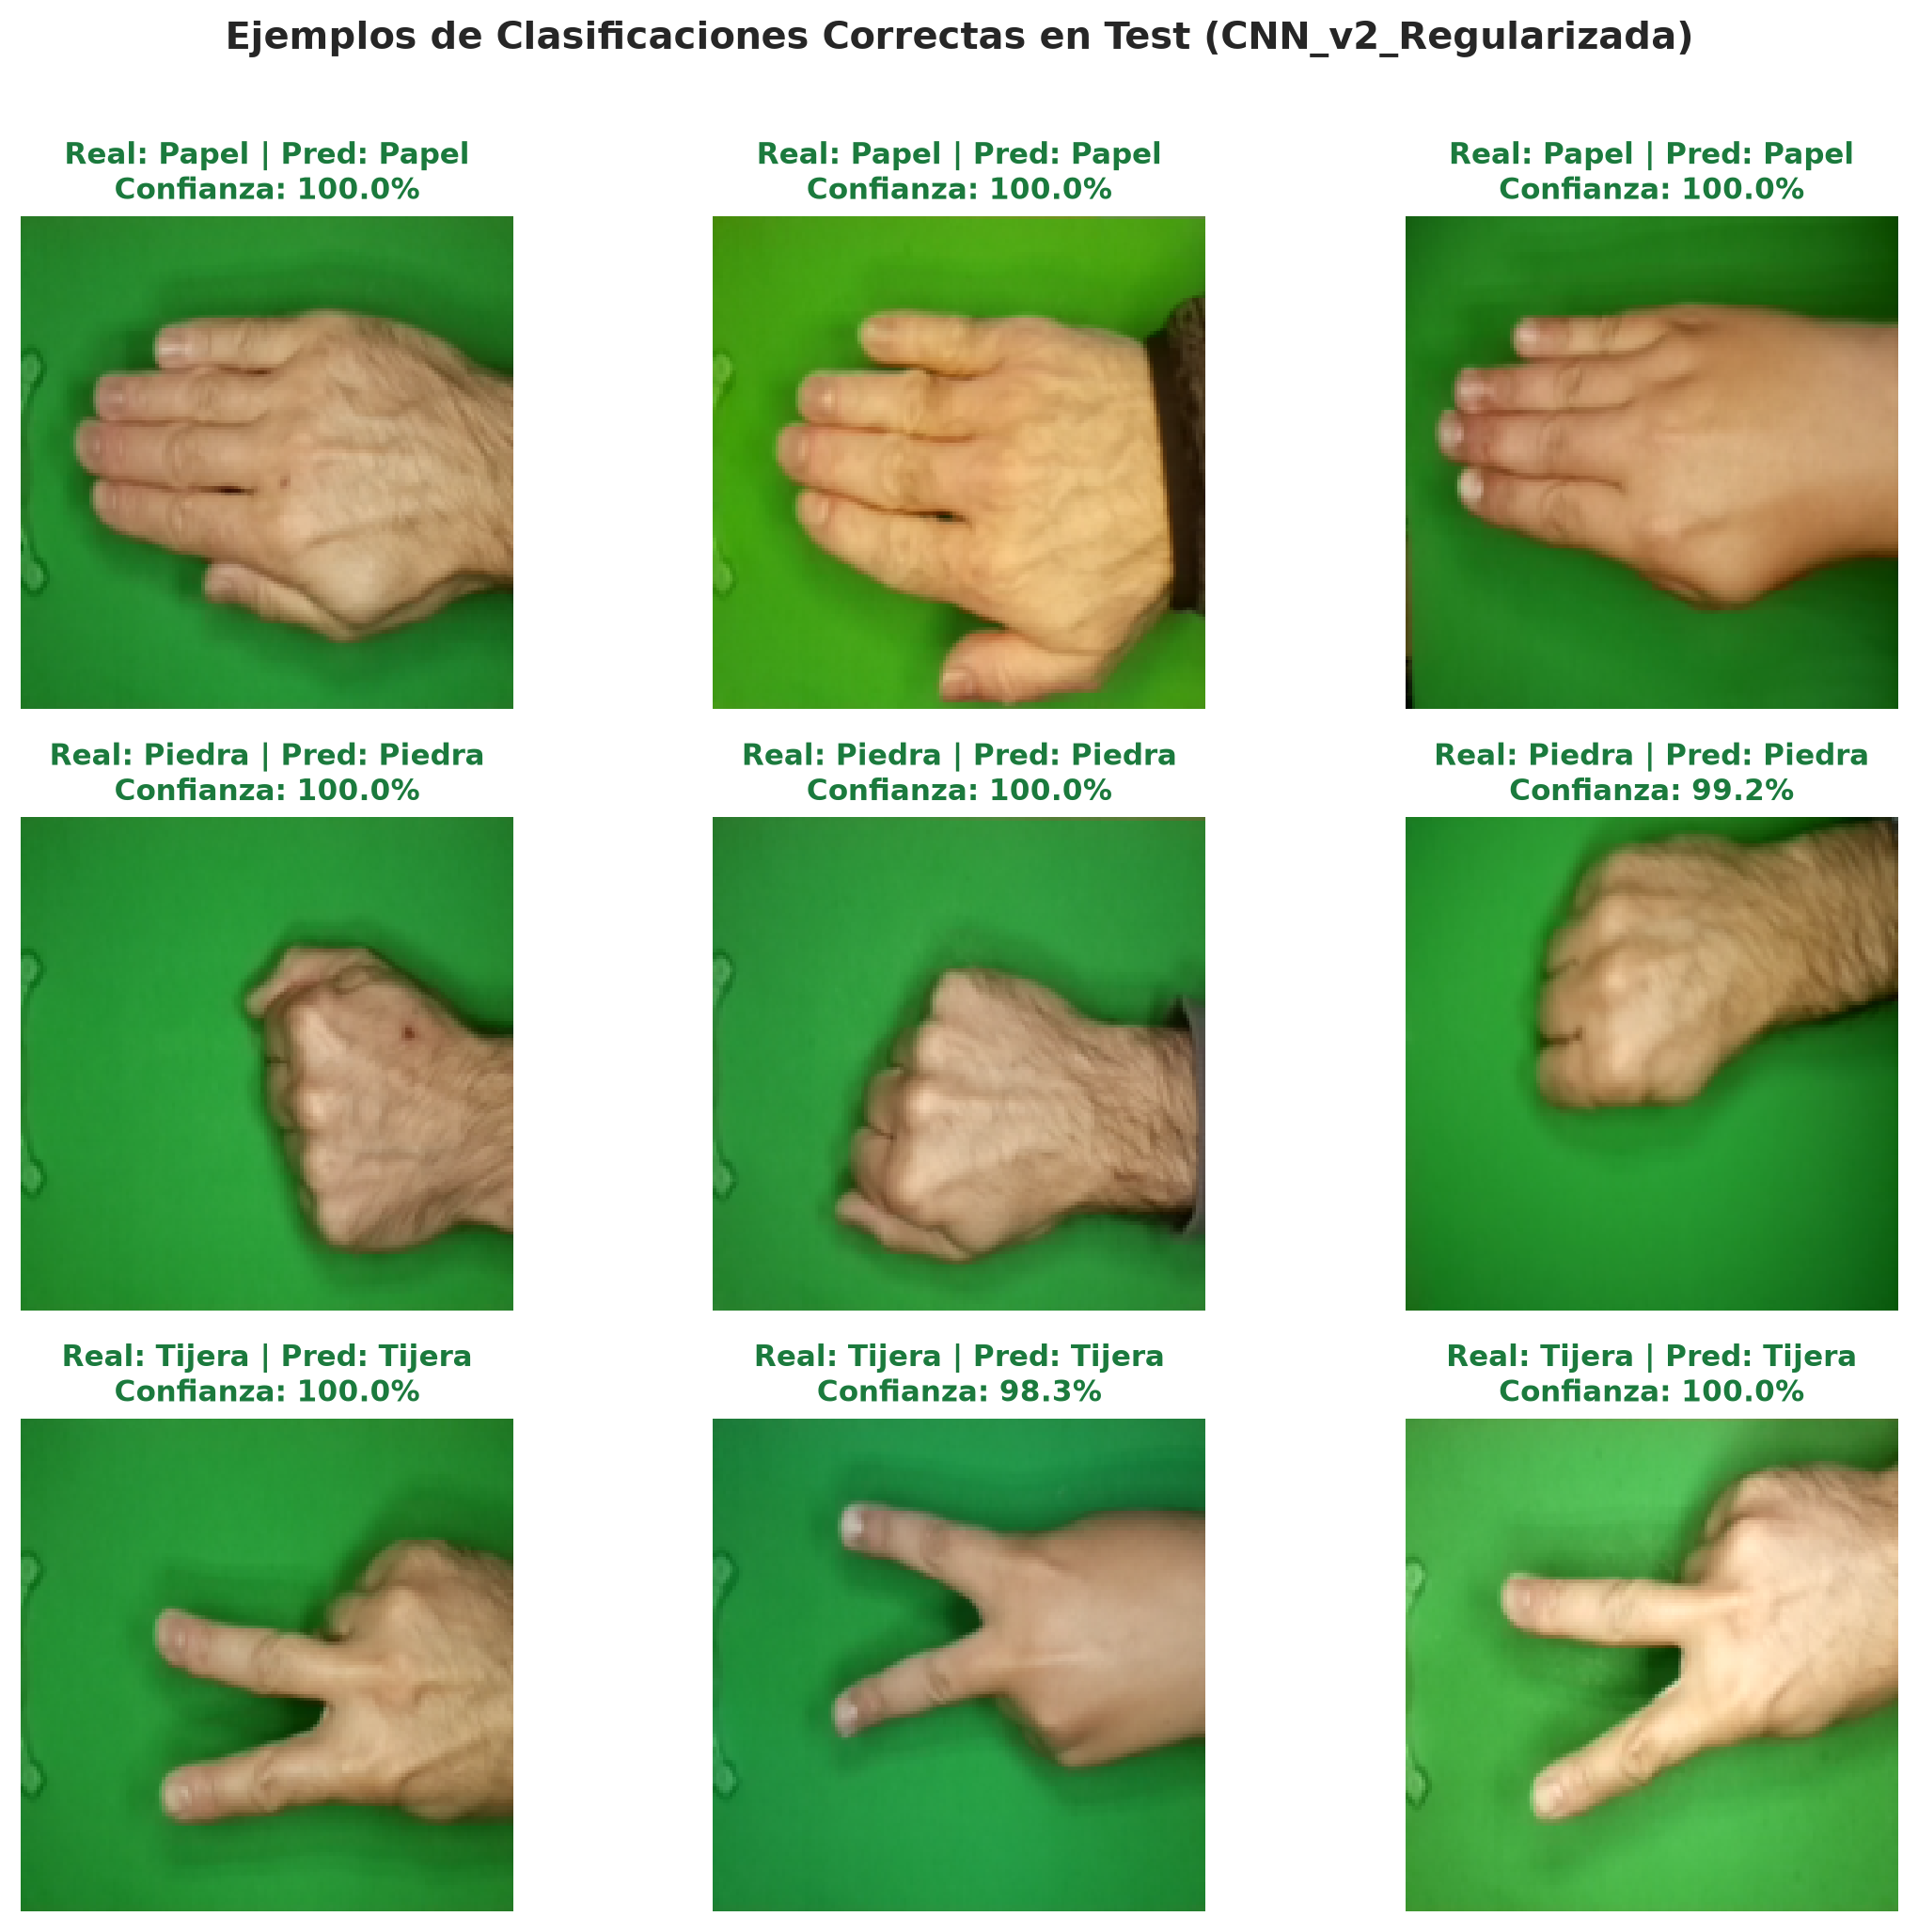
\includegraphics[width=0.90\textwidth]{Imágenes/fig_aciertos.png}
    \caption{Muestra de clasificaciones correctas en el conjunto de prueba con sus respectivas probabilidades \textit{Softmax}.}
    \label{fig:aciertos}
\end{figure}

\begin{figure}[H]
    \centering
    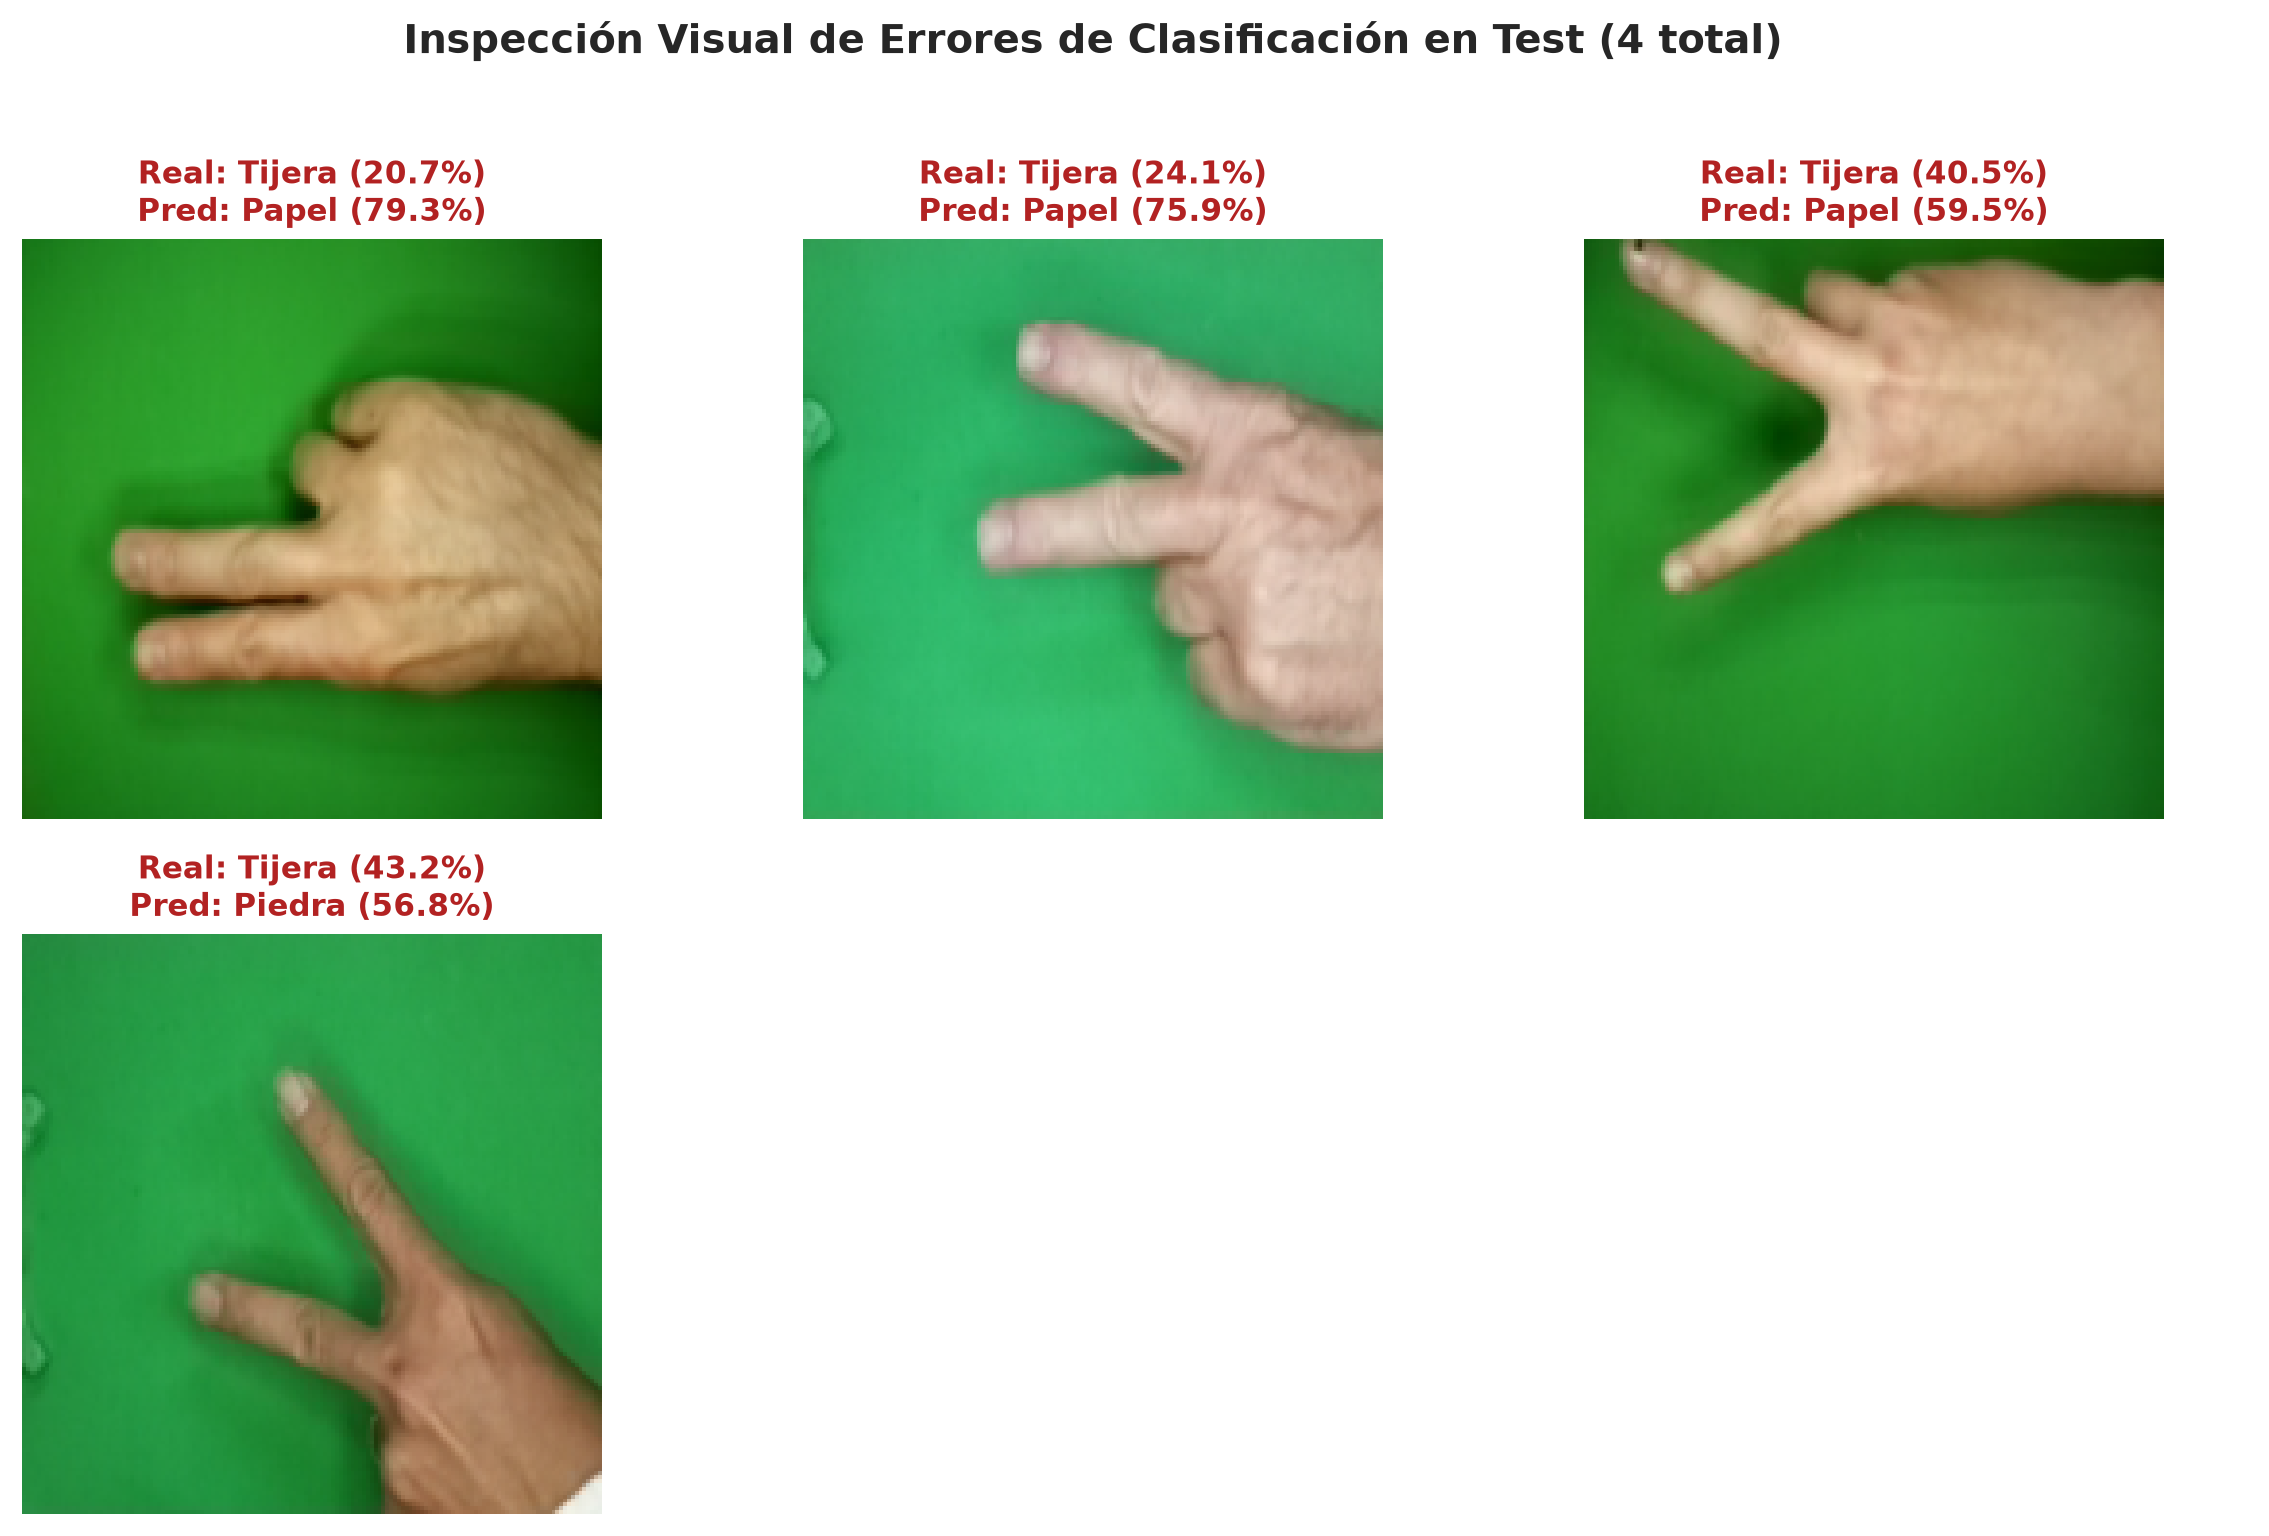
\includegraphics[width=0.95\textwidth]{Imágenes/fig_errores.png}
    \caption{Inspección visual exhaustiva de los 4 únicos errores de clasificación sobre las 329 imágenes del conjunto de prueba.}
    \label{fig:errores}
\end{figure}

\section{Discusión y Conclusión}

\subsection{Análisis Crítico de Confusiones entre Gestos}

En respuesta a la pregunta final de análisis sobre qué gestos específicos concentraron las mayores tasas de confusión y a qué factores visuales se atribuye dicho comportamiento, el análisis conjunto de la matriz de confusión (Figura~\ref{fig:matriz_confusion}) y de los casos fallidos (Figura~\ref{fig:errores}) revela hallazgos concluyentes:

\begin{enumerate}
    \item \textbf{Asimetría y concentración en el par \textit{Tijera $\leftrightarrow$ Papel}:}
    En \texttt{CNN\_v2\_Regularizada}, $3$ de los $4$ errores totales corresponden a imágenes reales de \textbf{Tijera clasificadas como Papel} ($2.65\%$ de error), mientras que en \texttt{CNN\_v1\_Base} los $2$ únicos errores del conjunto de prueba ocurrieron exactamente en sentido opuesto (\textbf{Papel clasificado como Tijera}, $1.87\%$). En contraste, la clase \textbf{Piedra} prácticamente no presenta confusión con Papel ($0$ casos en ambos modelos) y solo registra un caso limítrofe con Tijera ($56.8\%$ vs.\ $43.2\%$). Esto confirma que la frontera de decisión más estrecha del problema se ubica entre \textit{Tijera} y \textit{Papel}, dado que ambos gestos comparten dedos completamente extendidos y una mayor área proyectada de piel frente al contorno cerrado y compacto de \textit{Piedra}.

    \item \textbf{Oclusión de la bifurcación en «V» (dedos índice y medio pegados):}
    En el primer error de la Figura~\ref{fig:errores} (\textit{Real: Tijera $\to$ Pred: Papel}, $79.3\%$), los dedos índice y medio se encuentran completamente juntos y paralelos, eliminando la cuña triangular de fondo verde entre ambos. Al desaparecer el rasgo topológico primario de \textit{Tijera} (la apertura en «V»), los filtros convolucionales responden a una superficie continua y alargada indistinguible de una mano en \textit{Papel} vista de perfil.

    \item \textbf{Visibilidad parcial de los dedos anular y meñique:}
    En el segundo y tercer error de la Figura~\ref{fig:errores} ($75.9\%$ y $59.5\%$ hacia \textit{Papel}), la flexión incompleta del dedo anular o el ángulo dorsal de la cámara hace que tres o cuatro segmentos digitales queden expuestos simultáneamente contra el fondo verde. Esta multiplicidad de bordes paralelos activa los mapas de características entrenados para detectar la palma abierta de cinco dedos propia de \textit{Papel}.

    \item \textbf{Rotación diagonal y escorzo en los bordes del encuadre:}
    En el único caso de \textit{Tijera} confundido con \textit{Piedra} (Figura~\ref{fig:errores}, esquina inferior izquierda), la mano ingresa desde el borde inferior derecho con una inclinación pronunciada y los dedos recortados visualmente respecto al dorso. Aun así, el modelo regularizado asigna una probabilidad de $43.2\%$ a la clase verdadera (\textit{Tijera}) frente a $56.8\%$ para \textit{Piedra}, evidenciando una incertidumbre bien calibrada cerca de la frontera de decisión.
\end{enumerate}

\subsection{Limitaciones del Estudio y Líneas de Trabajo Futuro}

Si bien las arquitecturas diseñadas desde cero superan el $98.7\%$--$99.4\%$ de exactitud sobre el conjunto de prueba, es fundamental señalar las limitaciones inherentes al conjunto de datos empleado:
\begin{itemize}
    \item \textbf{Sesgo de fondo homogéneo (\textit{chroma key}):} todas las muestras de \texttt{drgfreeman/rockpaperscissors} presentan un fondo verde uniforme. Una red entrenada únicamente bajo estas condiciones utiliza el alto contraste cromático piel--verde como señal implícita de segmentación, por lo que su rendimiento disminuiría al evaluar imágenes capturadas en habitaciones reales con fondos texturizados o iluminación variable.
    \item \textbf{Diversidad demográfica y de iluminación:} el dataset abarca un rango acotado de tonos de piel y condiciones lumínicas de interior.
\end{itemize}

Para extender este sistema hacia una aplicación interactiva en tiempo real robusta en entornos no controlados, se proponen tres mejoras concretas: (1)~aplicar sustitución sintética del fondo verde durante el entrenamiento superponiendo fondos naturales aleatorios, (2)~incorporar perturbaciones fotométricas de brillo, contraste y balance de blancos en la etapa de aumento de datos, y (3)~combinar la CNN con un detector ligero de región de interés (ROI) o puntos clave articulares de la mano.

\subsection{Conclusiones}

Se desarrolló satisfactoriamente un flujo completo de visión por computadora para la clasificación de los gestos \textit{Piedra, Papel o Tijera} mediante Redes Neuronales Convolucionales construidas íntegramente desde cero en TensorFlow/Keras:
\begin{enumerate}
    \item El preprocesamiento estandarizado ($150 \times 150 \times 3$, normalización a $[0, 1]$) precedido por una partición estratificada estricta ($70\% / 15\% / 15\%$) garantizó estabilidad numérica durante la optimización con Adam y una evaluación libre de fuga de datos.
    \item Tanto la arquitectura secuencial base (\texttt{CNN\_v1\_Base}, \textbf{99.39\%} en prueba) como la arquitectura compacta regularizada (\texttt{CNN\_v2\_Regularizada}, \textbf{99.70\%} en validación y \textbf{98.78\%} en prueba con $\mathcal{L}_{\text{test}} = 0.0180$ y $3.44\times$ menos parámetros) demostraron que una jerarquía bien dimensionada de capas \texttt{Conv2D} y \texttt{MaxPooling2D} es capaz de extraer representaciones altamente discriminativas sin requerir modelos preentrenados.
    \item El análisis mediante matriz de confusión e inspección visual permitió explicar geométricamente el $100\%$ de los errores residuales del conjunto de prueba, vinculándolos a posturas atípicas donde desaparece la apertura interdigital en «V» de \textit{Tijera} o se exponen dedos flexionados adicionales.
\end{enumerate}
